\chapter*{Apple El Padre De La Revolución SmartPhone}
En este capítulo damos a conocer porque la compañía APPLE está tan destacada, sus grandes desarrollos, pasos e incluso su gran estabilidad económica a través del tiempo, lo 
cual hace interesante este capítulo. También las nuevas tecnologías y por supuesto de donde surgieron, quien las implementó y cómo fue su histórico desarrollo.  Nos basamos  
en que sabemos que APPLE fue el que inició la revolución de los ordenadores, reproductores mp3, celulares, Tablets gracias a su diseño novedoso y la gran garantía de 
seguridad tanto software como hardware. Indiscutiblemente Apple a sido el Thomas Alva Edison de nuestra era, el que revolucionó totalmente las vidas de todas las personas en 
todo el mundo, alguien se ha imagina el mundo sin celulares inteligentes, ni tablets? ...

\section*{Steve Jobs Una Mente Brillante}
Apple desde sus comienzos ha sido una de las empresas que ha revolucionado el mundo con sus invenciones en lo que dispositivos electrónicos respecta,  muestra de ello fue 
crear  la primera fábrica automatizada de computadores, la primera computadora personal, pionero en el uso de iconos y   ratón para controlar un computador eso era lo más 
innovador del momento a todo el mundo le encanto esta tecnología por y fue así como Apple tuvo su primer éxito Steve Jobs y Steve Wozniak sus creadores tenían tan solo 21 y 
26 años cuando lanzaron su primera computadora, la Apple1 y tuvo tanto éxito al cabo de 5 años la empresa había recaudado cientos de millones de dólares, luego de esto a la 
empresa se disparó como un cohete  en mayor parte gracias al ingenio y la creatividad de Steve Jobs. 

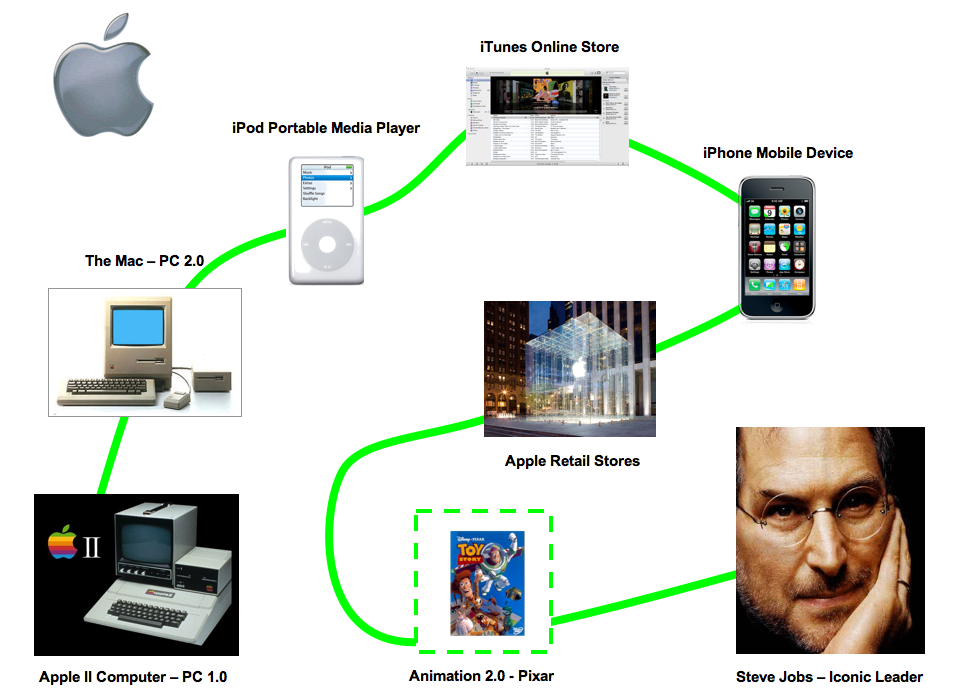
\includegraphics[scale=0.4]{img/cp08/img0801.png}

\section*{Inicios del iPhone}
Los ingenieros de Apple investigaron la mejor manera para crear el que sería el dispositivo insignia de la marca. Para ello tenia en mente una varias tecnologías novedosas 
para el momento una de ellas fue el gorilla glass que consiste en una pantalla muy resistente a golpes y rallones, pero esta tecnología podría aumentar los costos de 
producción del iphone ya que este cristal era muy caro de producir y hasta el momento no existía una empresa que fuera capaz  de producir este cristal a gran escala otra 
tecnología era un avanzado sistema operativo que fuera de la más la calidad Apple, además de esto el presidente de Apple Steve Jobs era un sujeto obsesionado con la 
presentación de su producto ya que para él la tecnología no solo tenía que ser funcional sino también tenía que ser bello y agradable al usuario, hasta el más mínimo 
detalle gráfico tenia era meticulosamente revisado para que este fuera el más llamativo sistema operativo del momento.

Toda la tecnología que implementó Apple en su celular tuvo un costo de 150 millones de dólares en investigaciones y diseño.

Bill Gates opinó al respecto sobre el iPhone dijo que este celular no iba a tener éxito ya que era muy caro y superaba por mucho el precio cualquier dispositivo  en el 
mercado hasta el momento. Para sorpresa de todos el Apple vendió 270 mil iPhones en las 30 primeras horas después de su lanzamiento y en el 2007 8 millones de iPhones se 
vendieron en Estados Unidos EEUU según la Entertainment Software Association. Luego de su éxito Apple lanzó varias versiones pero cada una de ellas ha tenido la 
particularidad de que todas sus configuraciones (botones) en el sistema operativo han estado en el mismo lugar con el fin de no confundir al usuario “cosa que no pasa con 
android”. Sin embargo muchoshans desertado del iPhone ya que su sistema operativo cerrado no le permite al usuario hacer modificaciones a su antojo y únicamente se puede 
interactuar a través de la aplicación iTunes "reproductor multimedia de Apple", continúa…

Apple vendió un millón de iPhone 3G en sus 3 primeros días de venta.

\section*{Características del iOS}
\subsection*{Seguridad}
Los virus y el malware ya no son solo problema de los ordenadores de mesa, también pueden atacar a dispositivos móviles. Apple se preocupa por la seguridad de iOS. El 
hardware están diseñados para defenderse de malware y virus, en cambio sabemos que iOS se ocupa de proteger la información personal. Y para garantizar aún más la seguridad 
también puedes poner una contraseña que impida el acceso no autorizado a tu dispositivo. Al usarla, iOS cifra tu correo electrónico y todas las apps de terceros para 
protegerlos.

\subsection*{Privacidad}

\subsection*{Accesibilidad Integral}

\subsection*{Interfaz}

